\documentclass[11pt, oneside]{article}
\usepackage[margin=1in]{geometry}
\geometry{letterpaper}
\usepackage{amssymb}
\usepackage[fleqn]{amsmath}
\usepackage[sharp]{easylist}
\usepackage{relsize}
\usepackage{graphicx}

\pagenumbering{gobble}              % No page numbering
\setlength{\parindent}{0em}         % No paragraph indenting
\setlength{\parskip}{0.5em}         % Paragraph spacing

\newcommand*{\begineasylist}{\begin{easylist}[itemize]\ListProperties(Style*=$\bullet$\quad, Style2*=\tiny$\blacksquare$\quad, Style3*=$\circ$\quad, Style4*=$\diamond$\quad, FinalSpace=1em, Space=0em, Space*=0em)}

\newcommand*{\begineasylistnumbered}{\begin{easylist}[enumerate]\ListProperties(Numbers=a, Space=0em, Space*=0em)}

\begin{document}

\section*{CS 247 Midterm Review}

\subsection*{ADT Design}
\begineasylist

# \textbf{Best practices}
## All data members should be \underline{private}
### Client accesses data through public methods
### Derived classes access data through protected methods
## Use \texttt{const} for function parameters whenever possible
## Accessor methods should be \texttt{const}

# \textbf{Default arguments}: only trailing parameters can have default values
## \texttt{function (int p1, int p2 = 0, int p3 = 1); }

# \textbf{Implicit type conversion}
## Prohibit by declaring constructor as \texttt{explicit}

# \textbf{Friends}: can access private members from outside of class
## Often used for streaming operators

# Operator overloading/special member functions
## \textbf{Default constructor}: generated by compiler if \& only if no constructors are declared

## \textbf{Destructor}: compiler default deallocates stack-based members, and calls destructors of member objects

## \textbf{Copy constructor}: compiler default performs \underline{shallow copy}

## \textbf{Assignment operator}: compiler default performs \underline{shallow copy}

## \textbf{Equality operator}: no compiler default

## \textbf{istream/ostream operator} (non-member functions): declare as friend

# \textbf{Rule of 3}:
## Destructor, copy constructor, assignment operator
## If one of these need to be defined, then all of them should be defined

# \textbf{Entity-based ADT}
## Prohibit assignment \& copy constructor
## Prohibit type conversion
## Compare pointer addresses for equality
## Mutable

# \textbf{Value-based ADT}
## Implement assignment \& copy constructor
## Implement equality \& comparisons
## Immutable

# \textbf{Header guard}: prevent errors when header declarations are included multiple times
## \texttt{\#ifndef CLASS\_H}\\
\texttt{\#define CLASS\_H}\\
\texttt{class Class \{ \ldots \};}\\
\texttt{\#endif \quad // Class}

# \textbf{Copy-swap idiom}: used to implement exception-safe assignment (e.g. \texttt{A = B;})
## Create local copy of \texttt{B} using copy constructor
## Swap contents of \texttt{A} and new copy of \texttt{B}
## \texttt{A} now has the contents of \texttt{B}; copy of \texttt{B} is deleted by destructor on function return

# \textbf{PImpl idiom}: instead of declaring internal workings (private data members) of a class in the public header file, declare in a \underline{nested class/struct in a separate file}
## ADT keeps a pointer to the Impl struct


\end{easylist}
\subsection*{Documentation}
\begineasylist

# \textbf{Interface specification}
## \textbf{Specification fields}: client's view of the object's fields (including private members)
## Preconditions:
### \textbf{Requires}: can throw exception immediately if preconditions are not satisfied
## Postconditions:
### \textbf{Modifies}: members that are changed
### \textbf{Ensures}: effects on the changed members (e.g. \texttt{this = this@pre + next})
### \textbf{Throws}: exceptions that may be thrown, and their conditions
### \textbf{Returns}: return value \& type
## Preconditions $\implies$ postconditions
## Spec A is \underline{stronger} than spec B (i.e. A $\implies$ B) if \& only if:
### A's preconditions are equal or weaker than B
### A's postconditions are equal or stronger than B
### A modifies equal or more objects than B
### A throws equal or fewer exceptions than B

# \textbf{Representation invariant}
## A predicate in an ADT that must be \underline{true at all times}
## Structural invariants
### e.g. two tree nodes cannot share the same child node; trees cannot have cycles
## Value invariants
### e.g. no duplicate data elements; a value cannot be null
## Should be checked \underline{on exit of constructor and mutators}

# \textbf{Abstraction function}
## Maps \underline{concrete values} to \underline{abstract values} in an ADT



\end{easylist}
\subsection*{Exceptions \& Smart Pointers}
\begineasylist

# \textbf{Assertion}: use to check a certain condition
## Terminates program immediately without changing its state

# \textbf{Exception}:
## Object representing an error that can be \emph{thrown} and \emph{caught}
## The call stack is popped/unwinded down to the nearest matching \texttt{catch} block
### Destructors of all stack objects are called
### i.e. heap objects are only handled properly if they are deleted in a stack object's destructor

# \textbf{Smart pointer}:
## Pointer encapsulated in a stack-based object
## Heap object is deleted in pointer object's destructor
### i.e. if exception is raised, heap object is deleted by the pointer's destructor
## \texttt{unique\_ptr<T>}: exclusive ownership of referent; ownership can be transferred
## \texttt{shared\_ptr<T>}: shared ownership of referent
### Object is deleted when the \# of \texttt{shared\_ptrs} pointing to it reaches 0
## \texttt{weak\_ptr<T>}: same as \texttt{shared\_ptr}, but doesn't contribute to reference count
### Need to check if expired, and then convert into \texttt{shared\_ptr} before dereferencing


\end{easylist}
\subsection*{RAII Idiom}
\begineasylist

# \textbf{Resource Acquisition is Initialization}: resource management is coupled with lifetime of object
## Allocate resource in constructor; deallocate resource in destructor
## \texttt{Class (param) : res\_( allocate (param); ) \{ \}}
## \texttt{$\sim$Class() \{ release (res\_); \}}


\end{easylist}
\newpage
\subsection*{UML (Unified Modelling Langauge)}
\begineasylist

# Attributes
## \texttt{[visibility] name: [type] [multiplicity] = [default value] \{property\}}
## e.g. \texttt{- playerName: string[1] = ""}
# Operations
## \texttt{[visibility] name (parameter list) : [return type] \{property\}}
## e.g. \texttt{+ getPlayerName ( playerId : int ) : string const}
## + public; - private; \# protected; \underline{static}; \emph{pure virtual}
## \texttt{property} = read-only (aka. const), query (aka. accessor), abstract, etc.

# Associations: physical or conceptual links between classes
## Classes being associated may have \underline{role names}
## Navigability: direction of association; e.g. A \emph{has} ($\rightarrow$) B

# Multiplicity: how many objects may fill the attribute/may be linked by an association
## $a$ = exactly $a$
## $m..n$ = between $m$ and $n$ (inclusive)
## $*$ = many (at least zero)
## $m..*$ = at least $m$

# Aggregate: a \underline{collection} of many members
## Member can belong to many collections, or exist independently
## Collection is \underline{not responsible} for its members

# Composition: a stricter collection of members
## Member cannot exist without its collection
## Member belongs to exactly one collection
## Collection is \underline{responsible} for its members

# Generalization = inheritance

# \textbf{Sequence diagrams}: describe how information is passed between objects (e.g. via function calls), throughout execution of a program
## Good at showing how different objects collaborate; not good at defining their behaviours precisely


\end{easylist}
\newpage
\subsection*{OOP Principles}
\begineasylist

# \textbf{Open Closed Principle}
## Modules should be \emph{open for extension} but \emph{closed for modification}
## ``Program to an interface, not an implementation''
## e.g. provide an abstract base class (may have default implementation) that can be extended by the client

# \textbf{Composition Over Inheritance}
## Composition = include base class in new subclass as a complex attribute
### i.e. ``has-a'' instead of ``is-a''
## Choose inheritance when subtyping, or when base class's original interface is required
## Choose composition for non-overriding extension or when new required interface is different from original, because the base component can be changed at runtime
## Composite object can \underline{delegate} operations to component objects (call the component's corresponding method)

# \textbf{Single-Responsibility Principle}
## Each changeable design decision (responsibility) should be encapsulated in a module
## An axis of change is an axis of change only if the changes occur; i.e. no need to separate responsibilities if they always change at different times

# \textbf{Liskov Substitutability Principle}
## A derived class must be substitutable for its base class
### Must accept the same messages (method signatures match the base class)
### Derived methods must \underline{require no more} (weaker or same preconditions) and \underline{promise no less} (stronger or same postconditions) than base class methods
#### Method return types match (or be a subtype) the base class
### Derived class must preserve properties of base class (e.g. invariant, performance)

# \textbf{Law of Demeter}
## An object should only ``talk to its neighbours'' (\underline{component composition})
## A method \texttt{C::m()} can only call methods of:
### C
### C's members
### m's parameters
### Any object constructed by A's methods
## Bad: \texttt{game->getPlayer()->getStatus()->getHP();}
## Good: \texttt{game->getPlayerHP();}


\end{easylist}
\newpage
\subsection*{Design Patterns}
\begineasylist

# \textbf{Inheritance}
## Parent class's methods are inherited by child classes
## Downside: not all subclasses may want to inherit parent behaviour
## Downside: code duplication

# \textbf{Strategy pattern}
## Allows the implementation of an algorithm/method to be changed at runtime \\(\underline{encapsulation of algorithm})
## Allows the algorithm to vary independently from clients that use it
## e.g. data structure holds an instance of base Strategy class, calls the algorithm/method (which is \emph{pure virtual} in base class)
### Concrete methods with differing behaviour are implemented in Strategy subclasses
### Strategy can be changed (to other subclasses) at runtime, changing the method's behaviour

\begin{figure}[!ht]
    \centering
    \includegraphics[width=0.8\textwidth]{res/strategy.png}
\end{figure}

# \textbf{Template pattern}
## \textbf{Template method} is a method in a base class that defines code structure but leaves \underline{holes} to be defined by subclasses
## Holes are operations defined as \emph{pure virtual} in the base class, but have varying implementations in subclasses

\begin{figure}[!ht]
    \centering
    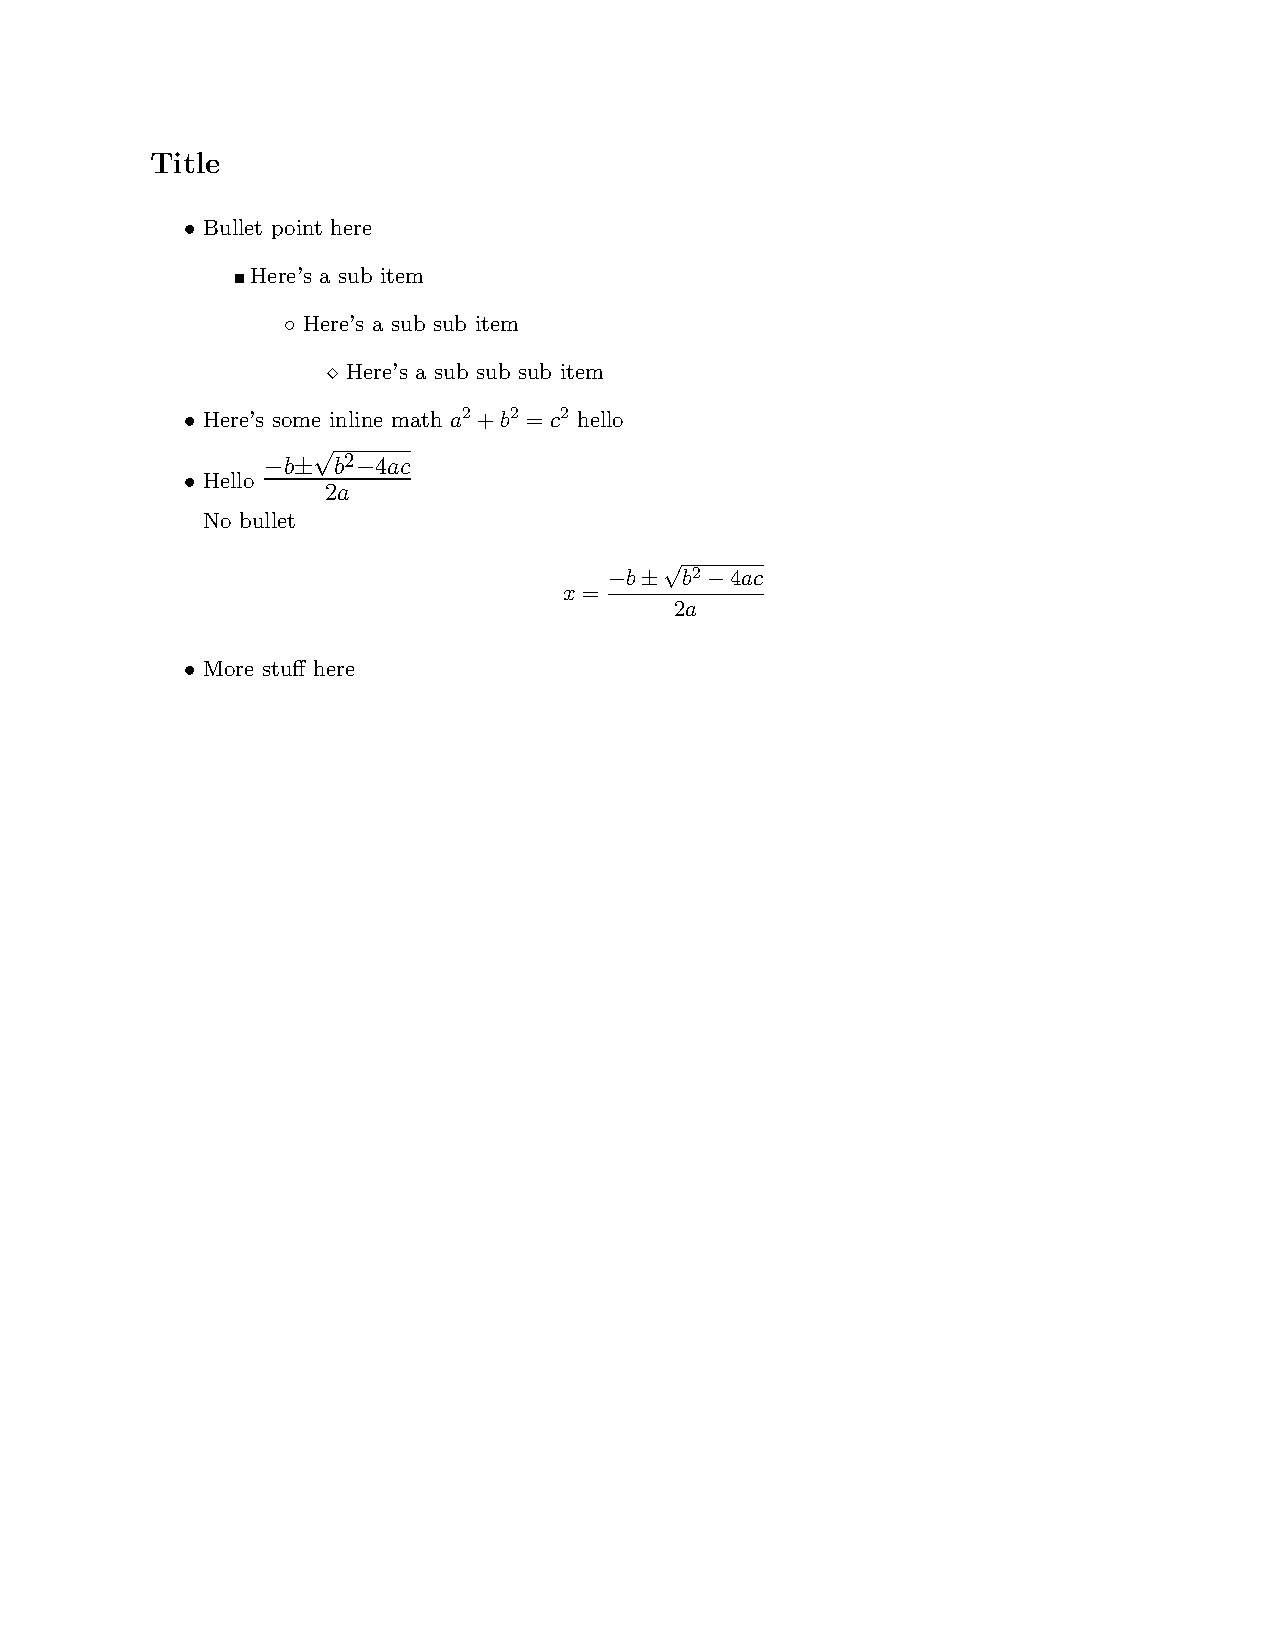
\includegraphics[width=0.6\textwidth]{res/template.png}
\end{figure}

\newpage

# \textbf{Adapter pattern}
## Adapter \underline{maps one interface to another}
## e.g. interface of an existing module does not match with a new module
## e.g. wrapping an existing data structure interface to create a new data structure

\begin{figure}[!ht]
    \centering
    \includegraphics[width=0.7\textwidth]{res/adapter.png}
\end{figure}

# \textbf{Facade pattern}
## Simplies and unifies classes and interfaces in a subsystem into only a high-level interface and hides individual interfaces within the subsystem
## Subsystem components and interfaces can be changed without affecting client

\begin{figure}[!ht]
    \centering
    \includegraphics[width=0.7\textwidth]{res/facade.png}
\end{figure}

# \textbf{Singleton pattern}
## Ensures \underline{only one instance} of a class can exist
## Private constructor; only instantiated through static \texttt{getInstance()} method

\newpage
# \textbf{Observer pattern}
## Subject $\rightarrow$ (one-to-many) Observers
## Subject can notify all subscribed observers to update
## Observers can subscribe/unsubscribe at runtime
## \textbf{Push model}: subject pushes state information to observers through \texttt{notify(State)}
## \textbf{Pull model}: subject notifies observers, who request information via subject's accessors
## \textbf{Loose coupling}: subjects and observers only know about each other's interfaces, not the concrete classes that implement them

\begin{figure}[!ht]
    \centering
    \includegraphics[width=0.5\textwidth]{res/observer.png}
\end{figure}

# \textbf{MVC pattern}
## UI code is abstracted into the \textbf{view}
### Composite pattern: all view elements use the same base class (uniform interface)

## \textbf{Controller} translates user input (from the view) into operations on the model
### Strategy pattern: controller provides the view with a strategy; controller behaviour can be changed by swapping for a different strategy

## \textbf{Model} holds data, state, and application logic
### Observer pattern: model = subject; views = observers; model sends out notification on state change, triggering views to update accordingly

# \textbf{Composite pattern}
## Components have a \underline{uniform interface}, and a \underline{union of leaf \& composite's services}
## Components are organized in a tree structure
## Set defaults in the base class for leaf-only or component-only operations (override in subclasses)

\begin{figure}[!ht]
    \centering
    \includegraphics[width=0.65\textwidth]{res/composite.png}
\end{figure}

# \textbf{Iterator pattern}
## Allows iteration through the elements of a collection without exposing representation
## Composite pattern iteration:
### Traverse tree using DFS (w/ a stack)
### Define iterator subclasses for both leaf and composite classes

\begin{figure}[!ht]
    \centering
    \includegraphics[width=0.7\textwidth]{res/iterator.png}
\end{figure}

# \textbf{Decorator pattern}
## Allows extra features to be added/removed to an object at runtime, by building wrappers
## Pass component into decorator to construct the original component w/ added functionality
### e.g. \texttt{Component* comp = new Component(); comp = new Decorator(comp);}

\begin{figure}[!ht]
    \centering
    \includegraphics[width=0.7\textwidth]{res/decorator.png}
\end{figure}

\newpage
# \textbf{Factory pattern}
## Uses the template pattern (encapsulates object creation)
## Abstract factory class defines the interface for object creation; concrete factory subclasses decide which object/how to construct

\begin{figure}[!ht]
    \centering
    \includegraphics[width=0.7\textwidth]{res/factory.png}
\end{figure}


\end{easylist}
\newpage
\subsection*{STL (Standard Template Library)}
\begineasylist

# \textbf{STL containers}
## Sequence containers: contiguous collection of variables; ordered (requires \texttt{operator<})

### \texttt{std::vector}
#### Wrapper around a C-style array (contiguous memory)
#### \underline{Reallocation invalidates pointers} to elements

### \texttt{std::deque}
#### Push/pop at front \emph{and} back
#### Growing the deque \underline{preserves pointers}

### \texttt{std::list}
#### Doubly-linked list; no random access

### \texttt{std::forward\_list}
#### Singly-linked list; no random access

### \texttt{std::array}
#### Fixed-size vector

## Container adapters: 
### \texttt{std::stack}, \texttt{std::queue}, \texttt{std::priority\_queue}
### Can specify which container to use (e.g. vector, deque etc.)
### \underline{Has (not inherits)} a private container member, to which operations are delegated
### \textbf{Adaptation}: extend a STL container by creating an adapter interface around it (as opposed to inheritance)
### \textbf{Private inheritance}: reuse base class's implementation without supporting its interface
#### Public \& protected API of base class are \underline{private} in the child class
#### Child class \underline{is not a subtype}; cannot be used polymorphically
#### Similar to adaptation

## Associative containers:
### Ordered containers: ordered based on value of key; implemented using BST
#### \texttt{std::[multi]map}, \texttt{std::[multi]set}

### Unordered containers: no particular ordering; implemented using hash tables
#### \texttt{std::unordered\_[multi]map}, \texttt{std::unordered\_[multi]set}

# \textbf{STL iterators}
## In decreasing hierarchy: 
## \textbf{Input/output iterator}: read-only/write-only, each location may only be visited once
## \textbf{Forward iterator}: can visit each location multiple times, can only move foward
## \textbf{Bidirectional iterator}: can iterate forwards and backwards
## \textbf{Random accessor iterator}: allows iterator arithmetic
## Use \texttt{back\_inserter}/\texttt{front\_inserter} to perform \texttt{push\_back()}/\texttt{push\_front()} on containers

# \textbf{STL algorithms}
## Use inserters when adding elements to containers (e.g. \texttt{std::copy} on vectors)
## Algorithms don't remove elements; ``removed'' elements are placed at the back of the container, and an iterator just past the last ``valid'' element is returned

# \textbf{Functors}
## Overload \texttt{operator()} to create function objects
### e.g. a binary function: \texttt{int operator() ( int a, int b) \{ return a + b; \}}

# \textbf{Function object adapters}
## \texttt{mem\_fun\_ref}/\texttt{mem\_fun}: convert a member function (of the container the algorithm is using) to a function object that can be passed to the algorithm
### Use \texttt{mem\_fun\_ref} for non-pointers (e.g. \texttt{string.length()})
### Use \texttt{mem\_fun} for pointers (e.g. \texttt{obj->size()})


\end{easylist}
\subsection*{Lambdas}
\begineasylist

# 


\end{easylist}

\end{document}
